%%%%%%%%%%%%%%%%%%%%%%%%%%%%%%%%%%%%%%%%%%%%%%%%%%%%%%%%%%%%%%%
%
% Welcome to Overleaf --- just edit your LaTeX on the left,
% and we'll compile it for you on the right. If you open the
% 'Share' menu, you can invite other users to edit at the same
% time. See www.overleaf.com/learn for more info. Enjoy!
%
%%%%%%%%%%%%%%%%%%%%%%%%%%%%%%%%%%%%%%%%%%%%%%%%%%%%%%%%%%%%%%%
\documentclass[12pt, a4paper]{article}
\usepackage[QX]{polski}
\usepackage[utf8]{inputenc}
\usepackage{latexsym}
\usepackage{underscore}
\usepackage{enumitem}
\usepackage{tgpagella}
\usepackage{tabularx}
\usepackage{array}
\usepackage{caption}
\usepackage{graphicx} % LaTeX package to import graphics
\usepackage[left=3cm,right=3cm,top=3cm,bottom=3cm]{geometry}
\graphicspath{{images/}} % configuring the graphicx package
\usepackage{booktabs}
\usepackage{unicode-math}
\usepackage{float}
\usepackage[colorlinks=true, linkcolor=black, citecolor=blue, urlcolor=blue]{hyperref}
% Code Handling
\usepackage{listings}
\usepackage{xcolor}
\usepackage[lighttt]{lmodern}
\newcolumntype{C}{>{\centering\arraybackslash}X}


%%%%%%%%%%%%%%%%%%%%%%%%%%%%%%%%%%%%%%%%%%%%%%%%%%%%%%%%%%%%%%%%%%%%%%%%%%%%%%%%%%%%%%%%%%%%%%%%%%%%%%%%%%%%%%%%%%%%%%%%%%%%%
% Verilog Code Style
%%%%%%%%%%%%%%%%%%%%%%%%%%%%%%%%%%%%%%%%%%%%%%%%%%%%%%%%%%%%%%%%%%%%%%%%%%%%%%%%%%%%%%%%%%%%%%%%%%%%%%%%%%%%%%%%%%%%%%%%%%%%%
\definecolor{verilogcommentcolor}{RGB}{104,180,104}
\definecolor{verilogkeywordcolor}{RGB}{49,49,255}
\definecolor{verilogsystemcolor}{RGB}{128,0,255}
\definecolor{verilognumbercolor}{RGB}{255,143,102}
\definecolor{verilogstringcolor}{RGB}{160,160,160}
\definecolor{verilogdefinecolor}{RGB}{128,64,0}
\definecolor{verilogoperatorcolor}{RGB}{0,0,128}

% Verilog style
\lstdefinestyle{prettyverilog}{
   language           = Verilog,
   commentstyle       = \color{verilogcommentcolor},
   alsoletter         = \$'0123456789\`,
   literate           = *{+}{{\verilogColorOperator{+}}}{1}%
                         {-}{{\verilogColorOperator{-}}}{1}%
                         {@}{{\verilogColorOperator{@}}}{1}%
                         {;}{{\verilogColorOperator{;}}}{1}%
                         {*}{{\verilogColorOperator{*}}}{1}%
                         {?}{{\verilogColorOperator{?}}}{1}%
                         {:}{{\verilogColorOperator{:}}}{1}%
                         {<}{{\verilogColorOperator{<}}}{1}%
                         {>}{{\verilogColorOperator{>}}}{1}%
                         {=}{{\verilogColorOperator{=}}}{1}%
                         {!}{{\verilogColorOperator{!}}}{1}%
                         {^}{{\verilogColorOperator{$\land$}}}{1}%
                         {|}{{\verilogColorOperator{|}}}{1}%
                         {=}{{\verilogColorOperator{=}}}{1}%
                         {[}{{\verilogColorOperator{[}}}{1}%
                         {]}{{\verilogColorOperator{]}}}{1}%
                         {(}{{\verilogColorOperator{(}}}{1}%
                         {)}{{\verilogColorOperator{)}}}{1}%
                         {,}{{\verilogColorOperator{,}}}{1}%
                         {.}{{\verilogColorOperator{.}}}{1}%
                         {~}{{\verilogColorOperator{$\sim$}}}{1}%
                         {\%}{{\verilogColorOperator{\%}}}{1}%
                         {\&}{{\verilogColorOperator{\&}}}{1}%
                         {\#}{{\verilogColorOperator{\#}}}{1}%
                         {\ /\ }{{\verilogColorOperator{\ /\ }}}{3}%
                         {\ _}{\ \_}{2}%
                        ,
   morestring         = [s][\color{verilogstringcolor}]{"}{"},%
   identifierstyle    = \color{black},
   vlogdefinestyle    = \color{verilogdefinecolor},
   vlogconstantstyle  = \color{verilognumbercolor},
   vlogsystemstyle    = \color{verilogsystemcolor},
   basicstyle         = \scriptsize\fontencoding{T1}\ttfamily,
   keywordstyle       = \bfseries\color{verilogkeywordcolor},
   numbers            = left,
   numbersep          = 10pt,
   tabsize            = 4,
   escapeinside       = {/*!}{!*/},
   upquote            = true,
   sensitive          = true,
   showstringspaces   = false, %without this there will be a symbol in the places where there is a space
   frame              = single
}


% This is shamelessly stolen and modified from:
% https://github.com/jubobs/sclang-prettifier/blob/master/sclang-prettifier.dtx
\makeatletter

% Language name
\newcommand\language@verilog{Verilog}
\expandafter\lst@NormedDef\expandafter\languageNormedDefd@verilog%
  \expandafter{\language@verilog}
  
% save definition of single quote for testing
\lst@SaveOutputDef{`'}\quotesngl@verilog
\lst@SaveOutputDef{``}\backtick@verilog
\lst@SaveOutputDef{`\$}\dollar@verilog

% Extract first character token in sequence and store in macro 
% firstchar@verilog, per http://tex.stackexchange.com/a/159267/21891
\newcommand\getfirstchar@verilog{}
\newcommand\getfirstchar@@verilog{}
\newcommand\firstchar@verilog{}
\def\getfirstchar@verilog#1{\getfirstchar@@verilog#1\relax}
\def\getfirstchar@@verilog#1#2\relax{\def\firstchar@verilog{#1}}

% Initially empty hook for lst
\newcommand\addedToOutput@verilog{}
\lst@AddToHook{Output}{\addedToOutput@verilog}

% The style used for constants as set in lstdefinestyle
\newcommand\constantstyle@verilog{}
\lst@Key{vlogconstantstyle}\relax%
   {\def\constantstyle@verilog{#1}}

% The style used for defines as set in lstdefinestyle
\newcommand\definestyle@verilog{}
\lst@Key{vlogdefinestyle}\relax%
   {\def\definestyle@verilog{#1}}

% The style used for defines as set in lstdefinestyle
\newcommand\systemstyle@verilog{}
\lst@Key{vlogsystemstyle}\relax%
   {\def\systemstyle@verilog{#1}}

% Counter used to check current character is a digit
\newcount\currentchar@verilog
  
% Processing macro
\newcommand\@ddedToOutput@verilog
{%
   % If we're in \lstpkg{}' processing mode...
   \ifnum\lst@mode=\lst@Pmode%
      % Save the first token in the current identifier to \@getfirstchar
      \expandafter\getfirstchar@verilog\expandafter{\the\lst@token}%
      % Check if the token is a backtick
      \expandafter\ifx\firstchar@verilog\backtick@verilog
         % If so, then this starts a define
         \let\lst@thestyle\definestyle@verilog%
      \else
         % Check if the token is a dollar
         \expandafter\ifx\firstchar@verilog\dollar@verilog
            % If so, then this starts a system command
            \let\lst@thestyle\systemstyle@verilog%
         \else
            % Check if the token starts with a single quote
            \expandafter\ifx\firstchar@verilog\quotesngl@verilog
               % If so, then this starts a constant without length
               \let\lst@thestyle\constantstyle@verilog%
            \else
               \currentchar@verilog=48
               \loop
                  \expandafter\ifnum%
                  \expandafter`\firstchar@verilog=\currentchar@verilog%
                     \let\lst@thestyle\constantstyle@verilog%
                     \let\iterate\relax%
                  \fi
                  \advance\currentchar@verilog by \@ne%
                  \unless\ifnum\currentchar@verilog>57%
               \repeat%
            \fi
         \fi
      \fi
      % ...but override by keyword style if a keyword is detected!
      %\lsthk@DetectKeywords% 
   \fi
}

% Add processing macro only if verilog
\lst@AddToHook{PreInit}{%
  \ifx\lst@language\languageNormedDefd@verilog%
    \let\addedToOutput@verilog\@ddedToOutput@verilog%
  \fi
}

% Colour operators in literate
\newcommand{\verilogColorOperator}[1]
{%
  \ifnum\lst@mode=\lst@Pmode\relax%
   {\bfseries\textcolor{verilogoperatorcolor}{#1}}%
  \else
    #1%
  \fi
}

\makeatother
%%%%%%%%%%%%%%%%%%%%%%%%%%%%%%%%%%%%%%%%%%%%%%%%%%%%%%%%%%%%%%%%%%%%%%%%%%%%%%%%%%%%%%%%%%%%%%%%%%%%%%%%%%%%%%%%%%%%%%%%%%%%%
% End Verilog Code Style
%%%%%%%%%%%%%%%%%%%%%%%%%%%%%%%%%%%%%%%%%%%%%%%%%%%%%%%%%%%%%%%%%%%%%%%%%%%%%%%%%%%%%%%%%%%%%%%%%%%%%%%%%%%%%%%%%%%%%%%%%%%%%



\title {\textbf{\fontsize{25}{29}\selectfont Laboratorium Techniki cyfrowej\\ 
\fontsize{17}{22}\selectfont \textit{Dokumentacja projektu}\\
\fontsize{17}{22}\selectfont \textit{Moduł generatora obrazu VGA}}}
\author{\fontsize{14}{10}\selectfont Szymon Miękina}
\date{\fontsize{14}{10}\selectfont Dominik Marek}

\begin{document}
\maketitle
\begin{figure}[h]
    \centering
    \includegraphics[scale=0.75]{images/agh_logo.jpg}
\end{figure}
\newpage
\tableofcontents
\section{Opis projektu}
Celem projektu było  napisanie programu ,wykorzystując język opisu sprzętu Verilog, który
umożliwi  wyświetlanie stabilnego obrazu za pomocą złącza VGA na programowalnym układzie
logicznym.

\section{Wykorzystany sprzęt}
Do realizacji projektu wykorzystano moduł Mimas Spartan6 rozbudowany o zewnętrzną pamięć IS61LV5128AL 512K x 8 HIGH-SPEED CMOS STATIC RAM.
\begin{figure}[h]
    \centering
    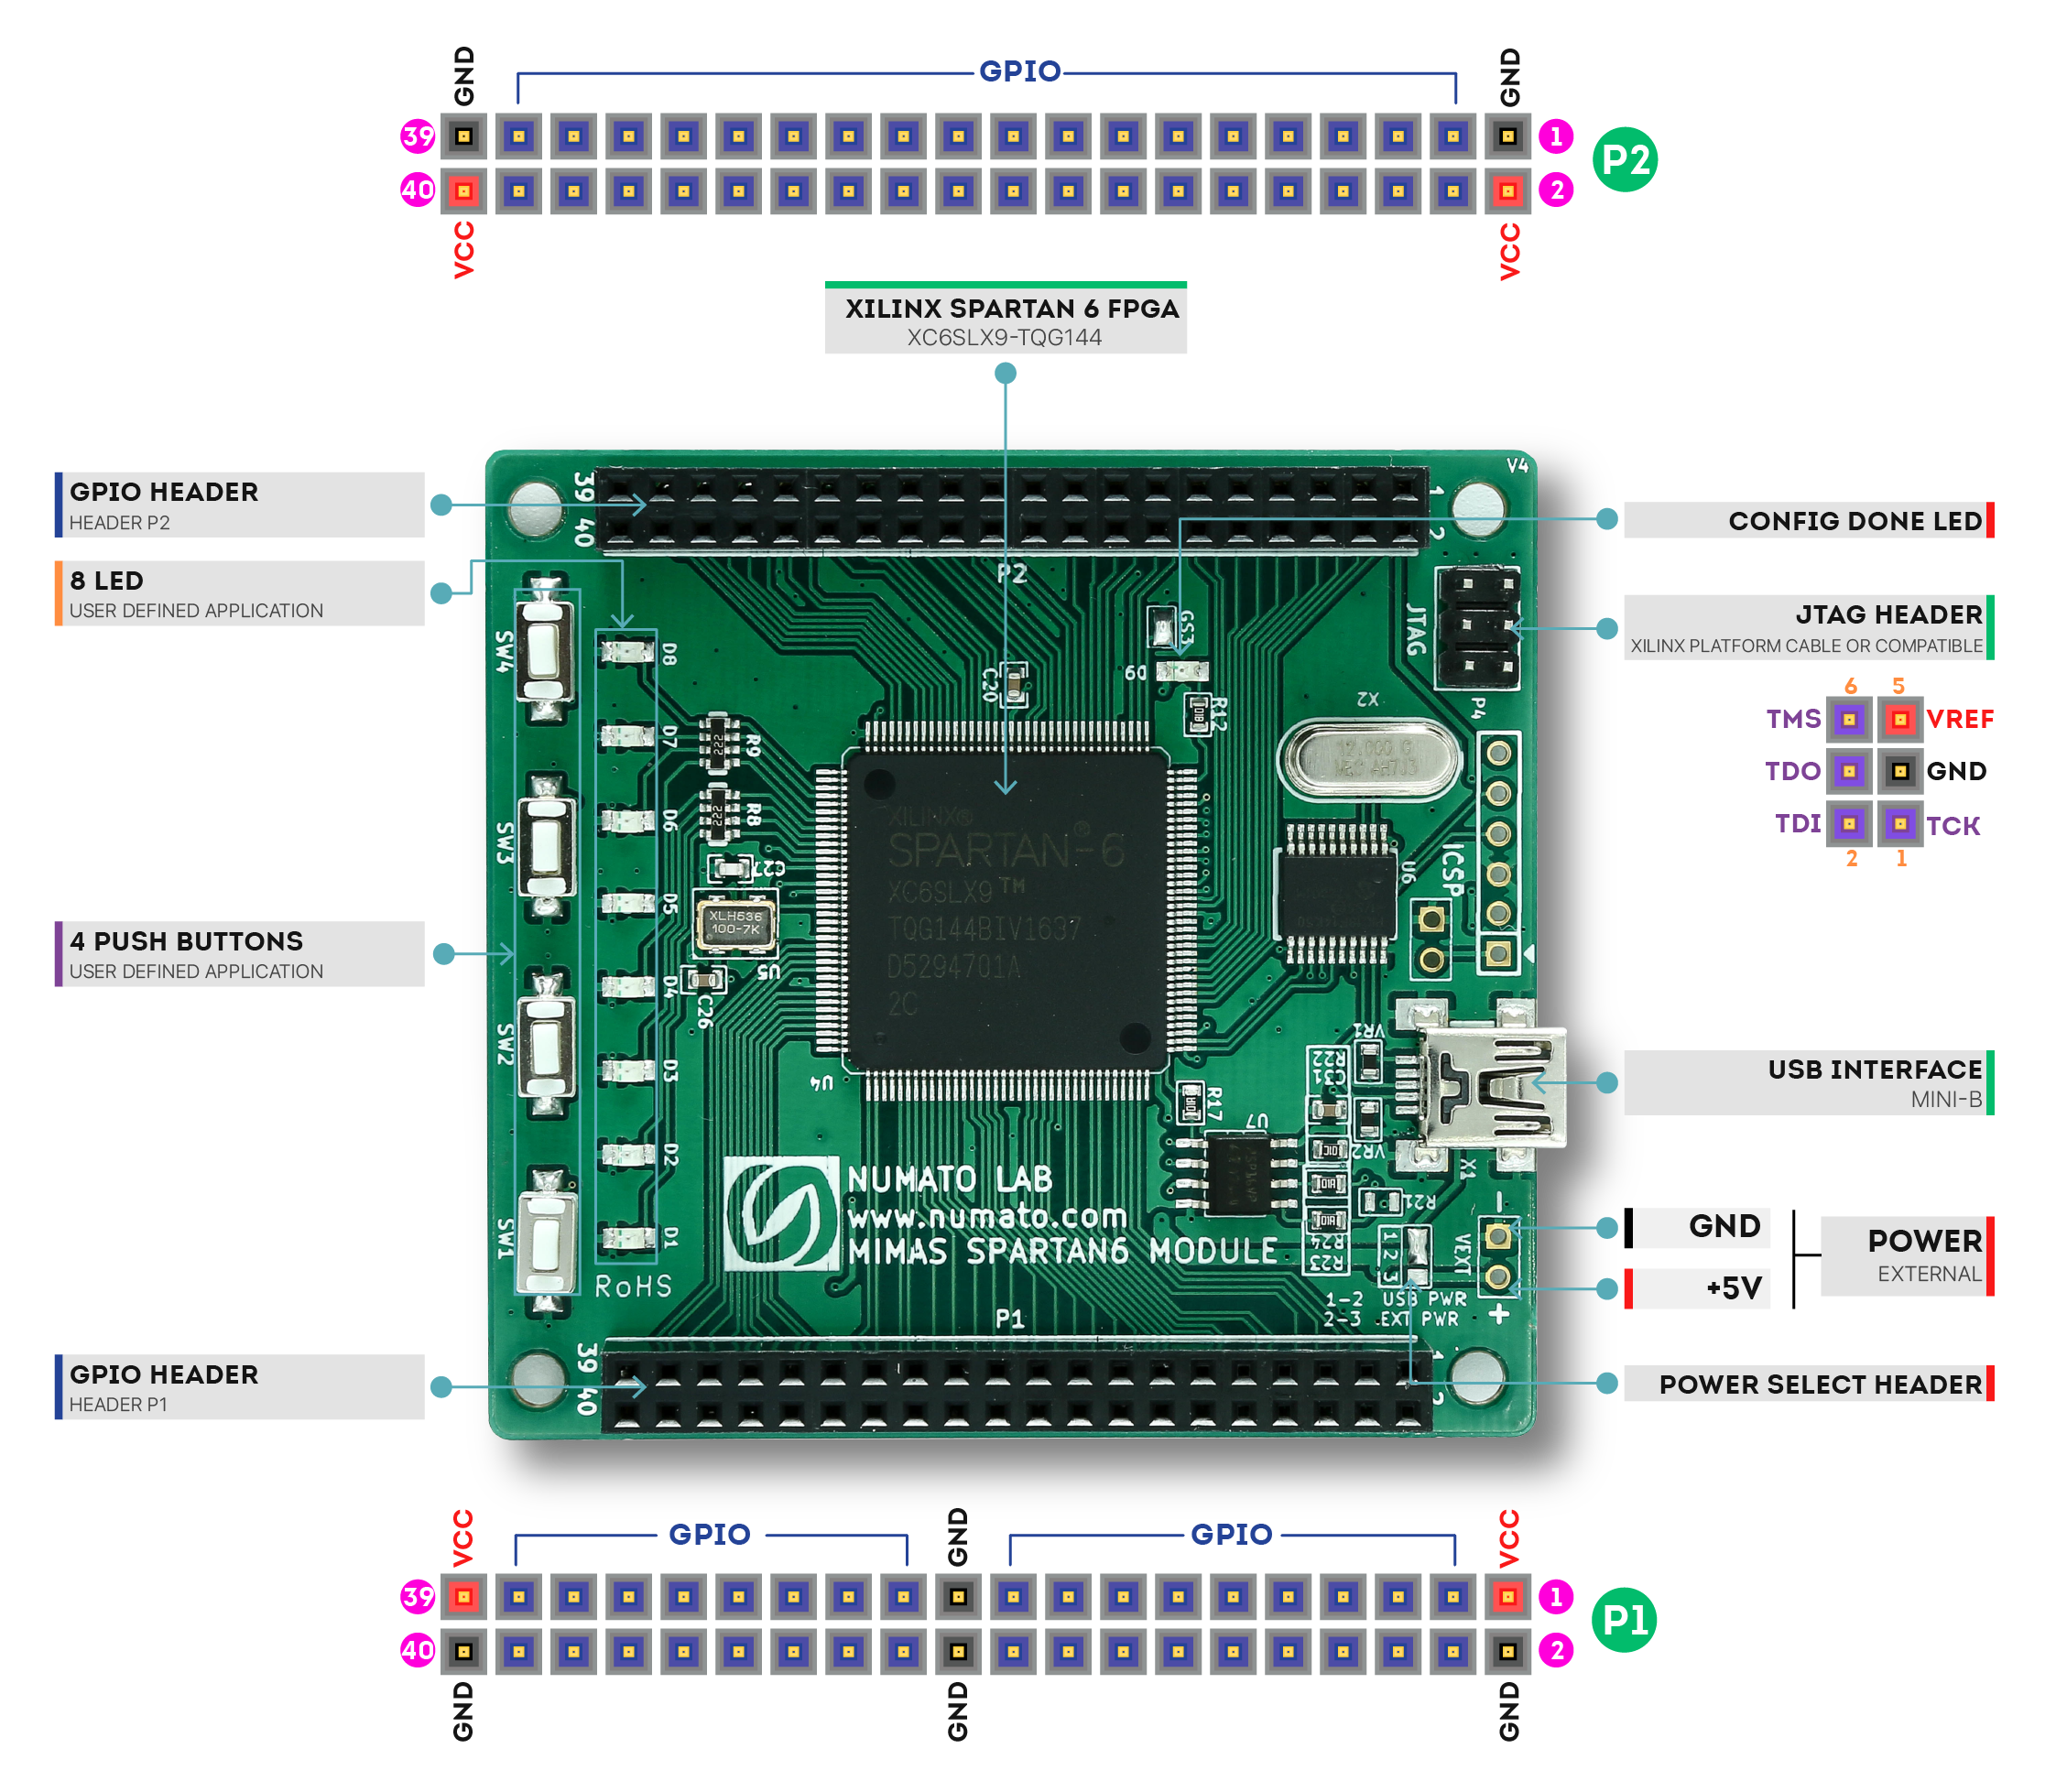
\includegraphics[scale=0.8]{images/spartan6_scheme.png}
     \caption{Płytka rozwojowa FPGA z układem Xilinx Spartan 6}
\end{figure}
\newpage
\section{Przygotwanie merytoryczne}
Przystępując do pracy zapoznaliśmy się z ze składnią, działaniem oraz użytecznymi w projkcie bibliotekami jezyka Verilog.Kolejnym krokiem było zaznajomienie się z dokumentacją oraz paramterami technicznymi sygnału VGA o rozdzielczości 640 na 480 i częstotliwości odświeżania 60Hz. 
\subsection{Sygnał w standardzie 640x480@60Hz}
W celu otrzymania sygnału o VGA o rozdzielczości 640 na 480 i odświeżaniu 60Hz, należało spełnić poniższe parametry sygnału o omawianym standardzie.
Dokładna ich realizacja została omówiona w rozdziale poświęconym poszczególnym modułom projektu.
\begin{table}[H]
    \centering
    \caption{General Timing Parameters}
    \begin{tabular}{|l|l|}
    \hline
    \textbf{Parameter} & \textbf{Value} \\ 
    \hline
    Screen refresh rate & 60 Hz \\
    Vertical refresh & 31.46875 kHz \\
    Pixel frequency & 25.175 MHz \\
    \hline
    \end{tabular}
\end{table}

\begin{table}[H]
    \centering
    \caption{Horizontal Timing (Line)}
    \begin{tabular}{|l|l|l|}
    \hline
    \textbf{Scanline part} & \textbf{Pixels} & \textbf{Time [$\mu s$]} \\ 
    \hline
    Visible area & 640 & 25.422045680238 \\
    Front porch & 16 & 0.63555114200596 \\
    Sync pulse & 96 & 3.8133068520357 \\
    Back porch & 48 & 1.9066534260179 \\
    Whole line & 800 & 31.777557100298 \\
    \hline
    \end{tabular}
\end{table}

\begin{table}[H]
    \centering
    \caption{Vertical Timing (Frame)}
    \begin{tabular}{|l|l|l|}
    \hline
    \textbf{Frame part} & \textbf{Lines} & \textbf{Time [ms]} \\ 
    \hline
    Visible area & 480 & 15.253227408143 \\
    Front porch & 10 & 0.31777557100298 \\
    Sync pulse & 2 & 0.063555114200596 \\
    Back porch & 33 & 1.0486593843098 \\
    Whole frame & 525 & 16.683217477656 \\
    \hline
    \end{tabular}
\end{table}

\begin{figure}[H]
    \centering
    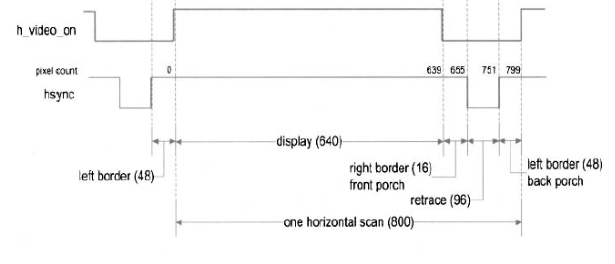
\includegraphics[scale=0.9]{images/horizontal_scan_lines.png}
     \caption{Schemat synchronizacji skanowania poziomego}
\end{figure}

\begin{figure}[H]
    \centering
    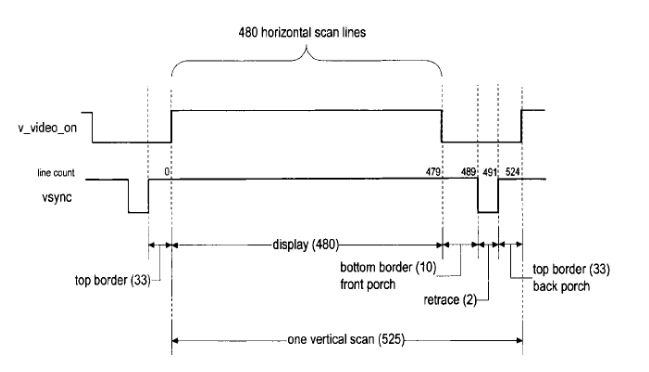
\includegraphics[scale=0.85]{images/vertical_scan_line.png}
     \caption{Schemat synchronizacji skanowania pionowego}
\end{figure}

\begin{figure}[H]
    \centering
    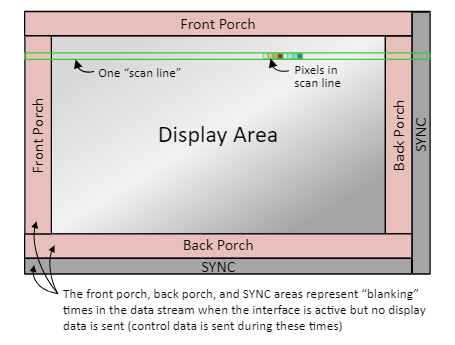
\includegraphics[scale=1.3]{images/display_control_signals.png}
     \caption{Sygnały sterujące wyświetlaniem obrazu.}
\end{figure}

\section{Realizacja projektu}
Po przeanalizowaniu wszystkich aspektów wymienionych wyżej, przystąpiliśmy do
projektowania programu, na który składa się jedynaście poniższych modułów.
\subsection{fifo.v}
Pierwszy moduł naszego projektu to bufor typu FIFO (First-In-First-Out),który służy do przechowywania danych w sposób, w którym dane, które pierwsze zostały umieszczone w buforze, są również pierwsze pobierane.
\begin{lstlisting}[style=prettyverilog,caption={Moduł fifo.v}]

module fifo #(
    parameter BUFSIZE = 16, // buffer size
    parameter IWIDTH = 4, // buffer index width
    parameter WWIDTH = 8 // memory word width
) (
    input wire[WWIDTH-1:0] DataIn,
    output reg[WWIDTH-1:0] DataOut,
    
    input wire ClkIn,
    input wire ClkOut,

    output wire IsFull,
    output wire IsEmpty
);

reg[WWIDTH-1:0] Buffer[BUFSIZE-1:0];
reg[IWIDTH-1:0] InIndex = 1'b0, OutIndex = 1'b0;

assign IsFull = InIndex + 1 == OutIndex;
assign IsEmpty = InIndex == OutIndex;

always @(posedge ClkIn) begin
    if (!IsFull) begin
        Buffer[InIndex] <= DataIn;
        InIndex <= InIndex < BUFSIZE-1 ? InIndex + 1 : 0;
    end
end

always @(posedge ClkOut) begin
    if (!IsEmpty) begin
	     DataOut <= Buffer[OutIndex];
        OutIndex <= OutIndex < BUFSIZE-1 ? OutIndex + 1 : 0;
    end
end

endmodule
\end{lstlisting}
Wejścia i wyjścia:
\begin{enumerate}
    \item \textbf{\fontsize{11}{10}\selectfont DataIn}: Dane wejściowe, które mają być zapisane do bufora FIFO.
    \item \textbf{\fontsize{11}{10}\selectfont DataOut}: Dane wyjściowe pobierane z bufora FIFO.
    \item \textbf{\fontsize{11}{10}\selectfont ClkIn}: Zegar dla operacji zapisu do bufora.
    \item \textbf{\fontsize{11}{10}\selectfont ClkOut}: Zegar dla operacji odczytu z bufora.
    \item \textbf{\fontsize{11}{10}\selectfont IsFull}: Sygnał wskazujący, czy bufor jest pełny.
    \item \textbf{\fontsize{11}{10}\selectfont IsEmpty}: Sygnał wskazujący, czy bufor jest pusty.
\end{enumerate}
\newline
Rejestry:
\begin{enumerate}
    \item \textbf{\fontsize{11}{10}\selectfont Buffer}: Tablica rejestrów przechowujących dane w buforze FIFO.
    \item \textbf{\fontsize{11}{10}\selectfont InIndex}: Licznik indeksu wskazujący na aktualną pozycję, do której będzie zapisywane dane.
    \item \textbf{\fontsize{11}{10}\selectfont OutIndex}: Licznik indeksu wskazujący na aktualną pozycję, z której będą odczytywane dane.
\end{enumerate}
W bloku always @(posedge ClkIn) następuje zapis danych do bufora FIFO. Jeśli bufor nie jest pełny (!IsFull), dane wejściowe (DataIn) są zapisywane do bufora na pozycji wskazywanej przez InIndex, a następnie InIndex jest inkrementowany.Gdy InIndex osiągnie maksymalny rozmiar bufora (BUFSIZE-1), wraca do początku.
Wraz z każdym narastającym zboczem zegara ClkOut następuje odczyt danych z bufora FIFO. Jeśli bufor nie jest pusty (!IsEmpty), dane są odczytywane z bufora z pozycji wskazywanej przez OutIndex, a następnie OutIndex jest inkrementowany. Jeśli OutIndex osiągnie maksymalny rozmiar bufora (BUFSIZE-1), wraca do początku.
\subsection{filter.v}
Poniższy moduł to filtr cyfrowy, który wykonuje proste przetwarzanie sygnału wejściowego SignalIn za pomocą sekwencji rejestrów opóźniających.
\begin{lstlisting}[style=prettyverilog,caption={Moduł filter.v}]
`timescale 1ns / 1ps

module filter #(
	parameter STAGES = 8
) (
	input wire ClkIn,
	input wire SignalIn,
	output reg SignalOut
);

reg[STAGES-1:0] Stages;

wire AllHigh = &Stages;
wire AllLow = ~|Stages;

always @(posedge ClkIn) begin
	Stages <= { Stages[STAGES-2:0], SignalIn };
	if (AllHigh) begin
		SignalOut <= 1'b1;
	end
	if (AllLow) begin
		SignalOut <= 1'b0;
	end
end

endmodule
\end{lstlisting}
\newpage
Wejścia i wyjścia;
\begin{enumerate}
    \item \textbf{\fontsize{11}{10}\selectfont ClkIn}: Zegar kontrolujący operacje w module.
    \item \textbf{\fontsize{11}{10}\selectfont SignalIn}: Sygnał wejściowy, który ma być przetwarzany przez filtr.
    \item \textbf{\fontsize{11}{10}\selectfont SignalOut}: Sygnał wyjściowy, który jest wynikiem przetwarzania przez filtr.
\end{enumerate}
\newline{}
Rejstry i połaczenia:
\begin{enumerate}
    \item \textbf{\fontsize{11}{10}\selectfont reg[STAGES-1:0] Stages}: Rejestry opóźniające, przez które przechodzi sygnał wejściowy.
 \item \textbf{\fontsize{11}{10}\selectfont\texttt{wire AllHigh = \& Stages}}: Połączenie sygnalizujące, czy wszystkie bity w Stages mają wartość 1.
    \item \textbf{\fontsize{11}{10}\selectfont\texttt{wire AllLow = \textasciitilde| Stages}}: Połączenie sygnalizujące, czy wszystkie bity w Stages mają wartość 0.
\end{enumerate}
W każdym cyklu zegara (ClkIn), wartość rejestru Stages jest aktualizowana o nową wartość sygnału wejściowego SignalIn, a następnie sprawdzane są warunki, czy wszystkie bity w rejestrze Stages są ustawione na wysoki (AllHigh) lub niski (AllLow) stan logiczny, aby odpowiednio ustawić sygnał wyjściowy SignalOut.
\subsection{spi.v}
W tym module zaimplenetowany został prosty odbiornik SPI( Serial Peripheral Interface) czyli szeregowy interfejs urządzeń peryferyjnych.W naszym przypadku będziemy go używać do komunikacji na lini mikrokontroler poszczególne komponenty układu.

\begin{lstlisting}[style=prettyverilog,caption={Moduł spi.v}]
module spi (
    input wire Clk,
    input wire Sclk,
    input wire Mosi,
    input wire CSel,
    output reg DataRecv,
    output reg[7:0] DataOut
);

reg[2:0] SclkSample;
always @(posedge Clk) SclkSample <= { SclkSample[1:0], Sclk };

wire SclkRise = SclkSample[2:1] == 2'b01;
wire SclkFall = SclkSample[2:1] == 2'b10;

reg[2:0] CSelSample;
always @(posedge Clk) CSelSample <= { CSelSample[1:0], CSel };

wire CSelActive = ~CSelSample[1];
wire CSelRise = CSelSample[2:1] == 2'b01;
wire CSelFall = CSelSample[2:1] == 2'b10;

reg[1:0] MosiSample;
always @(posedge Clk) MosiSample <= {MosiSample[0], Mosi};

wire MosiData = MosiSample[1];

reg[2:0] BitCnt = 3'b000;

reg[7:0] ByteDataRecv = 8'b00000000;

always @(posedge Clk) begin
    if (CSelFall) begin
	     BitCnt <= 3'b000;
	 end else if (SclkRise) begin
	     BitCnt <= BitCnt + 3'b001;
		  ByteDataRecv <= {ByteDataRecv[6:0], MosiData};
	 end
end

always @(posedge Clk) begin
	 if (~CSelActive && (BitCnt == 3'b000)) begin
	     DataRecv <= 1'b1;
        DataOut <= ByteDataRecv;
	 end else begin
	     DataRecv <= 1'b0;
	 end
end

endmodule
\end{lstlisting}
Wejścia i wyjścia:
\begin{enumerate}
    \item \textbf{\fontsize{11}{10}\selectfont input wire Clk}: Wejście zegara(Clock signal).
    \item \textbf{\fontsize{11}{10}\selectfont input wire Sclk}: Wejście zegara interfejsu SPI..
    \item \textbf{\fontsize{11}{10}\selectfont input wire Mosi}: Wejście danych z mikrokontrolera(Master Out Slave In)
    \item \textbf{\fontsize{11}{10}\selectfont input wire CSel}: Wejście selekcji układu (Chip Select).
    \item \textbf{\fontsize{11}{10}\selectfont output reg DataRecv}: Wyjście informujące,czy odbierana jest odpowiednia ilość danych.
    \item \textbf{\fontsize{11}{10}\selectfont output reg [7:0] DataOut}: Wyjście danych z układu (Master Out Slave In).\newline{}
\end{enumerate}

Rejestry wewnętrzne:

\begin{enumerate}
    \item \textbf{\fontsize{11}{10}\selectfont reg [2:0] SclkSample}: Rejestr do próbkowania sygnału zegara interfejsu SPI.
    \item \textbf{\fontsize{11}{10}\selectfont reg [2:0] CSelSample}: Rejestr do próbkowania sygnału wyboru interfejsu SPI.
     \item \textbf{\fontsize{11}{10}\selectfont reg [2:0] MosiSample}: Rejestr do próbkowania sygnału danych wyjściowych  interfejsu SPI.
    \item \textbf{\fontsize{11}{10}\selectfont reg [2:0] BitCnt}: Licznik bitów używany do śledzenia, który bit danych jest przesyłany
    \item \textbf{\fontsize{11}{10}\selectfont reg [7:0] ByteDataRecv}: Rejestr przechowujący dane przychodzące z linii Mosi.

\end{enumerate}


Moduł wykorzystuje próbkowanie zegara Sclk i sygnału wyboru układu CSel oraz sygnału danych wyjściowych Mosi, aby śledzić transmisję danych w interfejsie SPI.Licznik BitCnt jest inkrementowany przy każdym zboczu narastającym zegara systemowego Clk, gdy CSel jest aktywne i Sclk jest w stanie wysokim. Otrzymane bity są zapisywane w ByteDataRecv. Następnie jeśli sygnału selekcji układu jest nieaktywny oraz otrzymano już cały bajt danych, sygnał DataRecv jest ustawiany na 1, co sygnalizuje gotowość danych. Dane są przekazywane przez DataOut.W przeciwnym razie sygnał DataRecv jest ustawiany na 0.

\subsection{spitest.v}
Moduł spitest jest testbenchem dla dwóch modułów: spi i vcmd, pozwalającym na symulację interakcji między nimi.
\begin{lstlisting}[style=prettyverilog,caption={Moduł spitest.v}]
`timescale 1ns / 1ps

module spitest;

	// Inputs
	reg Clk = 1'b0;
	reg Sclk = 1'b0;
	reg Mosi = 1'b0;
	reg CSel = 1'b1;

	// Outputs
	wire DataRecv;
	wire [7:0] DataOut;
	
	initial forever
		#2 Clk <= ~Clk;

	// Instantiate the Unit Under Test (UUT)
	spi UUT (
	   .Clk(Clk),
		.Sclk(Sclk), 
		.Mosi(Mosi), 
		.CSel(CSel), 
		.DataRecv(DataRecv), 
		.DataOut(DataOut)
	);
	
	task send_byte(input time PulseTime, input [7:0] Byte);
		begin
			CSel = 1'b0;
			// for (j = 0; j < 8; j = j + 1)
			#PulseTime;
			send_pulse(PulseTime, (Byte>>7) & 1);
			send_pulse(PulseTime, (Byte>>6) & 1);
			send_pulse(PulseTime, (Byte>>5) & 1);
			send_pulse(PulseTime, (Byte>>4) & 1);
			send_pulse(PulseTime, (Byte>>3) & 1);
			send_pulse(PulseTime, (Byte>>2) & 1);
			send_pulse(PulseTime, (Byte>>1) & 1);
			send_pulse(PulseTime, (Byte>>0) & 1);
			Sclk = 1'b0;
			#PulseTime;
			CSel = 1'b1;
			#PulseTime;
		end
	endtask
	
	task send_pulse(input time PulseTime, input Data);
		begin
			Mosi = Data;
			Sclk = 1'b0;
			#PulseTime;
			Sclk = 1'b1;
			#PulseTime;
		end
	endtask

	initial begin
		// Wait 100 ns for global reset to finish
		#100;
        
		// Add stimulus here
		send_byte(40, 8'b01000001);
		send_byte(40, 8'b11000000);
		send_byte(40, 8'b11000000);
		send_byte(40, 8'b11000000);
	
		#500;
		
		send_byte(40, 8'b01000001);
		send_byte(40, 8'b11000000);
		send_byte(40, 8'b11000000);
		send_byte(40, 8'b11000000);
	end
      
endmodule
\end{lstlisting}
Na początku definiowane są wejścia (Sclk, Mosi, CSel) i wyjścia (DataRecv, DataOut) dla modułu spi, oraz wejścia (CmdDataIndex) i wyjścia (CmdMemAddr, CmdDataOut, CmdDataRdy) dla modułu vcmd. Następnie zdefiniowane są dwa zadania testowe.

Zadanie \texttt{send_byte} przyjmuje dwie wartości wejściowe: PulseTime, który określa czas trwania impulsu, oraz Byte, który jest bajtem do wysłania przez interfejs SPI. Najpierw linia CSel jest ustawiana na stan niski, co sygnalizuje rozpoczęcie transmisji. Następnie każdy bit bajtu Byte jest przesyłany pojedynczo poprzez wywołanie zadania \texttt{send_pulse} dla każdego bitu. Po wysłaniu wszystkich bitów, linia CSel ponownie jest ustawiana na stan wysoki, sygnalizując zakończenie transmisji. Zadanie \texttt{send_pulse} ustawia linię Mosi na wartość Data, ustawia zegar Sclk na stan wysoki, czeka przez określony czas PulseTime, ustawia zegar Sclk na stan niski i ponownie czeka przez PulseTime, symulując pojedynczy impuls zegara oraz przesyłanie jednego bitu danych przez linię MOSI.

W sekcji initial ustawiane są początkowe wartości sygnałów oraz oczekuje się 100 ns na zakończenie resetowania. Po zakończeniu resetowania generowane są impulsy SPI, symulujące wysyłanie danych do urządzenia. Każda wysyłka danych poprzedzona jest krótką przerwą (\#500), co symuluje niewielkie opóźnienie między kolejnymi operacjami.

\subsection{vbuffer.v}
Moduł vbuffer odczytuje piksele za pomocą modułu zarządzania pamięcią i zapisuje je do bufora wyjściowego.
Piksele są przechowywane w formacie RGB222 (6 bitów na piksel), co oznacza, że każde 4 piksele mogą być przechowywane w 3 bajtach pamięci.Ponieważ kontroler pamięci wymaga zapisania czterech pikseli za jednym raz, powyższa operacja pozwala zredukować kosztowne odczytanie z pamięci, jednak tym samym indeksy kolumn muszą zaczynać się od wielokrotności czwórki.Dane w pamięci wideo są zorganizowane w blokach pikseli, gdzie każdy blok składa się z 4 pikseli. Aby zidentyfikować dany blok pikseli, używane są wskaźniki bloków, które składają się z indeksu linii i indeksu poziomego bloku. Indeks linii odpowiada numerowi wiersza na ekranie, natomiast indeks poziomego bloku wskazuje, który blok od początku wiersza jest wybrany. Rozpoczęcie numeru kolumny wyświetlania można obliczyć, mnożąc indeks poziomego bloku przez cztery.

\begin{lstlisting}[style=prettyverilog,caption={Moduł vbuffer.v}]
`timescale 1ns/1ps

// TODO: add double buffer for memory reading
module vbuffer #(
    parameter IWIDTH = 2, // index width
    parameter BPP = 6, // bits per pixel
    parameter PSIZE = 4 // pixels stored
) (
    input wire PixelClk,
    input wire ReqWrite,
    input wire Blank,
    input wire[IWIDTH-1:0] ReadIndex,
    input wire[IWIDTH-1:0] WriteIndex,
    input wire[7:0] DataIn,
    output reg[BPP-1:0] VideoOut
);

parameter WSIZE = BPP * PSIZE / 8;

reg[7:0] WriteBuffer[WSIZE-1:0];
reg[BPP-1:0] PixelBuffer[PSIZE-1:0];

always @(posedge PixelClk) begin
	 if (ReadIndex == 1'b0) begin
	 	  PixelBuffer[3] = WriteBuffer[2][5:0];
		  PixelBuffer[2] = { WriteBuffer[1][3:0], WriteBuffer[2][7:6] };
		  PixelBuffer[1] = { WriteBuffer[0][1:0], WriteBuffer[1][7:4] };
		  PixelBuffer[0] = WriteBuffer[0][7:2];
	 end
	 
    if (Blank) begin
	     VideoOut = 1'b0;
    end
    else VideoOut = PixelBuffer[ReadIndex];
end
    
always @(negedge ReqWrite) begin
    WriteBuffer[WriteIndex] = DataIn;
end

endmodule
\end{lstlisting}
Wejścia i wyjścia:
\begin{enumerate}
    \item \textbf{\fontsize{11}{10}\selectfont input wire PixelClk}: Wejście zegara systemowego (Clock signal).
    \item \textbf{\fontsize{11}{10}\selectfont input wire ReqWrite}: Sygnał żądania zapisu danych do bufora.
    \item \textbf{\fontsize{11}{10}\selectfont input wire Blank}: Sygnał wygaszania.
    \item \textbf{\fontsize{11}{10}\selectfont input wire [IWIDTH-1:0] ReadIndex}: Indeks odczytu danych.
    \item \textbf{\fontsize{11}{10}\selectfont input wire [IWIDTH-1:0] WriteIndex}: Indeks zapisu danych.
    \item \textbf{\fontsize{11}{10}\selectfont input wire [BPP-1:0] DataIn}: Dane wejściowe do zapisu
    \item \textbf{\fontsize{11}{10}\selectfont output reg [BPP-1:0] VideoOut}: Dane wyjściowe.
\end{enumerate}
Obliczamy zmienną WSIZE, która reprezentuje całkowitą liczbę bajtów potrzebnych do zapisania liczby pikseli podanych w paramterze PSIZE przy formacie wymagającym BBP bitów na piksel.Następnie tworzymy dwa bufory.Pierwszy  WriteBuffer określa tablicę rejestrów, która będzie służyć do przechowywania danych wejściowych .Natomiast w zmiennej PixelBuffer będziemy przechowywać piksele do odczytu.
W każdym cyklu zegara jesli synał odczytu jest nieaktywny w buforze PixelBuffer pod adresami reprezentującymi kolejene piksele  zapisujemy dane odpowiadające danemu pikselowi z rejestru WriteBuffer. Jeśli sygnał wygaszania jest w stanie wysokim to dane wyjściowe ustawiamy na zero w przeciwnym razie przypisujemy do nich dane znadujące się w buforze odczytu pod adresem ReadIndex.
Finalnie z każdym opadjącym zboczem sygnału repreznetującego żądanie zapisu w buforze WriteBuffer pod indeksem WriteIndex zapisujemy dane wejściowe.
\subsection{vcmd.v}
Moduł Video Command Processor (VCDM) będzie maszyną stanów odpowiednio przetwarzającą otrzymane sygnały z interfesju komunikacji (spi).
\begin{lstlisting}[style=prettyverilog,caption={Moduł vcmd.v}]
`include "fifo.v"

module vcmd (
  input wire ByteRecvClk,
  input wire DataModeEnable,
  input wire[7:0] ByteIn,
  input wire ReadOutClk,
  
  output wire HasReadData,
  output wire[18:0] AddrOut,
  output wire[7:0] DataOut
);

// TODO finish vcmd data

localparam Noop = 8'h00;
localparam SetAddr = 8'h01;

localparam ReadCmdId = 4'h0;
localparam SetAddrPage = 4'h4;
localparam SetAddrHigh = 4'h5;
localparam SetAddrLow = 4'h6;

reg[18:0] NextAddr = 1'b0;
reg[18:0] ReadAddr = 1'b0;

reg[3:0] State = 1'b0;

wire BufferOverflow;
wire BufferUnderflow;
wire PushByte = ~BufferOverflow && DataModeEnable && ByteRecvClk;
assign HasReadData = ~BufferUnderflow;

wire _BufferOverflow;
wire _BufferUnderflow;

fifo #(
  .BUFSIZE(8),
  .WWIDTH(8)
) DataFIFO (
  .DataIn(ByteIn),
  .ClkIn(PushByte),
  .DataOut(DataOut),
  .ClkOut(ReadOutClk),
  .IsEmpty(BufferUnderflow),
  .IsFull(BufferOverflow)
);

fifo #(
  .BUFSIZE(8),
  .WWIDTH(19)
) AddrFIFO (
  .DataIn(NextAddr),
  .ClkIn(PushByte),
  .DataOut(AddrOut),
  .ClkOut(ReadOutClk),
  .IsEmpty(_BufferUnderflow),
  .IsFull(_BufferOverflow)  
);

function [3:0] SelectCmd(input[7:0] CmdId);
  begin
    case (CmdId)
      Noop: SelectCmd = ReadCmdId;
      SetAddr: SelectCmd = SetAddrPage;
    endcase
  end
endfunction

always @(posedge ByteRecvClk) begin
  if (DataModeEnable) begin
    NextAddr <= NextAddr + 1'b1;
  end else begin
    case (State)
      ReadCmdId: State <= SelectCmd(ByteIn);
      SetAddrPage: begin
        ReadAddr[18:16] <= ByteIn[2:0];
        State <= SetAddrHigh;
      end
      SetAddrHigh: begin
        ReadAddr[15:8] <= ByteIn;
        State <= SetAddrLow;
      end
	   SetAddrLow: begin
        ReadAddr[7:0] <= ByteIn;
        NextAddr <= ReadAddr;		  
        State <= ReadCmdId;
	   end
      default: State <= ReadCmdId;
    endcase
  end
end

endmodule
\end{lstlisting}
Wejścia i wyjścia:
\begin{enumerate}
     \item \textbf{\fontsize{11}{10}\selectfont input wire ByteRecvClk}: Zegar używany do synchronizacji odbieranych bajtów.
    \item \textbf{\fontsize{11}{10}\selectfont input wire DataModeEnable}:  Sygnał sterujący trybem pracy, informujący moduł o odbieraniu danych lub poleceń.
    \item \textbf{\fontsize{11}{10}\selectfont input wire[7:0] ByteIn}: Sygnał reprezentujący konkretne polecenie.
    \item \textbf{\fontsize{11}{10}\selectfont input wire ReadOutClk}: Zegar używany do synchronizacji danych odczytanych z FIFO.
     \item \textbf{\fontsize{11}{10}\selectfont output wire [7:0] HasReadData}: Sygnał informujący, czy dostępne są dane do odczytu z FIFO.
     \item \textbf{\fontsize{11}{10}\selectfont output reg [18:0] AddrOut}: Adres pamięci wyjściowej.
     \item \textbf{\fontsize{11}{10}\selectfont output wire [7:0] DataOut}: Dane wyjściowe
\end{enumerate}
Rejestry i połączenia:
\begin{enumerate}
    \item \textbf{\fontsize{11}{10}\selectfont reg [18:0] NextAddr}: 18-bitowy rejestr przechowujący następny adres pamięci, który za zostać zapisany W FIFO.
    \item \textbf{\fontsize{11}{10}\selectfont reg [18:0] ReadAddr}: 18-bitowy rejestr przechowujący adres pamięci, który aktualnie za zostać zapisany W FIFO
    \item \textbf{\fontsize{11}{10}\selectfont reg[3:0] State}: 4-bitowy rejestr przechowujący aktualny stan maszyny stanowej.
    \item \textbf{\fontsize{11}{10}\selectfont BufferOverflow}: Sygnał informujący o przepełnieniu bufora kolejki FIFO.
    \item \textbf{\fontsize{11}{10}\selectfont BufferOverflow}: Sygnał informujący o tym czy bufor kolejki FIFO jest pusty.
    \item \textbf{\fontsize{11}{10}\selectfont PushByte}: Sygnał sterujący zapisem danych do kolejki FIFO.
    \item \textbf{\fontsize{11}{10}\selectfont \texttt{assign HasReadData = \(\sim\)BufferUnderflow}}: Przpisanie do sygnału HasReadData negacji wartości sygnału BufferUnderflow, informujące tym samym czy w kolejce znajdują się dane do odczytu.


\end{enumerate}
Konfigurujemy dwa bufory FIFO jeden do przechowywania danych wejściowych a drugi dla adresów pamięci.
Następnie uwtorzona funkcja SelectCmd jest używana do mapowania otrzymanego identyfikatora komendy przekazywanej jak paramter modułu (CmdId) na odpowiedni kod stanu przeznaczony dla  maszyny stanowej.
Z każdym narastającym zboczem zegara ByteRecvClk jeśli moduł jest w trybie odbierania danych(sygnał DataModeEnable jest aktywny) następuje inkrementacja NextAddr. W przeciwnym przypadku w zależności od obecnego stanu reprezentowanego przez zmienną State wykonywane są następujące czynności:
\begin{enumerate}[label={\textbullet}]
    \item \textbf{\fontsize{12}{10}\selectfont ReadCmdId}: 
    Stan, w którym oczekujemy się na otrzymanie nowego polecenia. Po otrzymaniu 
    polecenia, aktulizowany jest obecny stan(State).

    \item \textbf{\fontsize{12}{10}\selectfont SetAddrPage}: 
    Jeśli aktualny stan to ustawianie adresu strony, to trzy najmłodsze bity otrzymanego bajtu (ByteIn[2:0]) są przypisywane do odpowiednich bitów ReadAddr[18:16], które określają te bity adresu.Następnie State jest aktualizowane do kolejnego stanu SetAddrHigh.

    \item \textbf{\fontsize{12}{10}\selectfont SetAddrHigh}:
     Otrzymane dane są przypisywane do bitów ReadAddr[15:8], które określają część wysoką adresu.Następnie jak kolejny stan ustawiony zostaje SetAddrLow, aby w kolejnym kroku odczytać pozostałą część adresu.
    
     \item \textbf{\fontsize{12}{10}\selectfont SetAddrLow}:
     W tym stanie otrzymane dane są przypisywane do bitów ReadAddr[7:0], które określają część niską adresu. Następnie NextAddr jest aktualizowany do wartości ReadAddr, co pozwala na rozpoczęcie kolejnej operacji zapisu na właściwym adresie. Stan (State) jest również ustawiany ponownie na ReadCmdId, aby przygotować moduł do odczytu kolejnej komendy.

\end{enumerate}

Finalnie z każdym opadającym zoboczem sygnału HoldUpadte, jeśli sygnał informujący o gotowości do odczytu danych jest aktywny,wówczas jak adres pamięci wyjściowej ustawiamy aktulanie wykorzystywany adres pamięci(MemAddr), a do buforu wyjściowego pod kolejnymi indeksami zapisujemy dane z rejstru DataBuffor.

W poniższej tabeli zostały przedstawione poszczególne komendy oraz działania wziązane z nimi.
\begin{center}
\begin{table}[h]
\centering
\caption{Odniesienia poleceń}
\begin{tabular}{|c|c|p{6cm}|}
\hline
\textbf{Instrukcja} & \textbf{Format} & \textbf{Opis} \\
\hline
NOOP & 0x00 & Brak czynności \\
\hline
BUFSWAP & 0x01 & Zacznij odczytywać następny blok pikseli z innego bufora \\
\hline
SETNOINC & 0x10 & Nie inkrementuj wskaźnika bloku po każdym zapisaniu \\
\hline
SETHINC & 0x11 & Zwiększ poziomy wskaźnik bloku po każdym zapisaniu \\
\hline
SET0 & 0x12 & Zresetuj wskaźniki bloków do (0,0) \\
\hline
SETX & 0x2X,0xXX & Ustaw kolumnę 'X' wskaźnika docelowego bloku \\
\hline
SETY & 0x3Y,0xYY & Ustaw linię 'Y' wskaźnika docelowego bloku \\
\hline
WRITE1U & 0x40,0xPP,0xPP,0xPP,0xPP & Zapisz rozpakowany blok pikseli \\
\hline
WRITE1P & 0x41,0xPP,0xPP,0xPP & Zapisz spakowany blok pikseli \\
\hline
WRITENU & 0x42,0xNN,0xNN,0xPP,... & Zapisz N ($<65,536$) rozpakowanych bloków pikseli \\
\hline
WRITENP & 0x43,0xNN,0xNN,0xPP,... & Zapisz N ($<65,536$) spakowanych bloków pikseli \\
\hline
\end{tabular}
\end{table}
\end{center}
\newpage
\subsection{vcmdtest.v}
Moduł VideoCommandProcessorTest to testbench dla dwóch modułów: spi i vcmd. Pozwala on  przeprowadzenie symulacji interakcji między wymienionymi modułami.
\begin{lstlisting}[style=prettyverilog,caption={Moduł vcmdtest.v}]
`timescale 1ns / 1ps

module vcmdtest;

	// SPI 

	// Inputs
	reg Sclk;
	reg Mosi;
	reg CSel;

	// Outputs
	wire DataRecv;
	wire [7:0] DataOut;

	// Instantiate the Unit Under Test (UUT)
	spi Spi (
		.Sclk(Sclk), 
		.Mosi(Mosi), 
		.CSel(CSel), 
		.DataRecv(DataRecv), 
		.DataOut(DataOut)
	);
	
	task send_byte(input time PulseTime, input [7:0] Byte);
		begin
			CSel = 1'b0;
			send_pulse(PulseTime, (Byte>>7) & 1);
			send_pulse(PulseTime, (Byte>>6) & 1);
			send_pulse(PulseTime, (Byte>>5) & 1);
			send_pulse(PulseTime, (Byte>>4) & 1);
			send_pulse(PulseTime, (Byte>>3) & 1);
			send_pulse(PulseTime, (Byte>>2) & 1);
			send_pulse(PulseTime, (Byte>>1) & 1);
			send_pulse(PulseTime, (Byte>>0) & 1);
			CSel = 1'b1;
		end
	endtask
	
	task send_pulse(input time PulseTime, input Data);
		begin
			Mosi = Data;
			Sclk = 1'b1;
			#PulseTime;
			Sclk = 1'b0;
			#PulseTime;
		end
	endtask      

	// VCMD

	// Inputs
	reg [1:0] DataIndex;

	// Outputs
	wire [17:0] CmdMemAddr;
	wire [7:0] CmdDataOut;
	wire CmdDataRdy;

	// Instantiate the Unit Under Test (UUT)
	vcmd UUT (
		.CmdRecv(DataRecv), 
		.CmdIn(DataOut), 
		.MemAddr(CmdMemAddr), 
		.DataOut(CmdDataOut), 
		.DataIndex(CmdDataIndex), 
		.DataRdy(CmdDataRdy)
	);
	
	initial begin
		// Initialize Inputs
		Sclk = 0;
		Mosi = 0;
		CSel = 0;
		DataIndex = 0;

		// Wait 100 ns for global reset to finish
		#100;
        
		// Add stimulus here
		// Very fast SPI clock (50MHz)
		send_byte(10, 8'b01000001);
		send_byte(10, 8'b11000000);
		send_byte(10, 8'b11000000);
		send_byte(10, 8'b11000000);
		
		// Small delay between next pixel write
		#160;
		
		// Another byte at next location
		send_byte(10, 8'b01000001);
		send_byte(10, 8'b00000011);
		send_byte(10, 8'b00000011);
		send_byte(10, 8'b00000011);
	end
      
endmodule
\end{lstlisting}

Na początku definiowane są wejścia (\texttt{Sclk}, \texttt{Mosi}, \texttt{CSel}) i wyjścia (\texttt{DataRecv}, \texttt{DataOut}) dla modułu \texttt{spi}, oraz wejścia (\texttt{CmdDataIndex}) i wyjścia (\texttt{CmdMemAddr}, \texttt{CmdDataOut}, \texttt{CmdDataRdy}) dla modułu \texttt{vcmd}. Następnie definiowane są dwa zadania testowe. \texttt{Send_byte} przyjmuje dwie wartości wejściowe: \texttt{PulseTime}, który określa czas trwania impulsu, oraz \texttt{Byte}, który jest bajtem do wysłania przez interfejs SPI.W zadaniu \texttt{send_byte} najpierw ustawiana jest linia \texttt{CSel} na stan niski (\texttt{CSel = 1'b0}), co sygnalizuje urządzeniu docelowemu, że rozpoczyna się transmisja. Następnie każdy bit bajtu \texttt{Byte} jest przesyłany pojedynczo poprzez wywołanie zadania \texttt{send\_pulse}. Dla każdego bitu wywoływane jest \texttt{send\_pulse} z odpowiednim bitem przesuniętym do prawej ((\texttt{Byte>>i}) \& 1), gdzie \texttt{i} to numer bitu. Po wysłaniu wszystkich bitów, linia \texttt{CSel} ponownie ustawiana jest na stan wysoki (\texttt{CSel = 1'b1}), sygnalizując zakończenie transmisji.Zadanie \texttt{send_pulse} ustawia linie \texttt{Mosi} na wartość \texttt{Data}, ustawia zegar \texttt{Sclk} na stan wysoki, czeka przez określony czas \texttt{PulseTime}, ustawia zegar \texttt{Sclk} na stan niski i ponownie czeka przez \texttt{PulseTime}. To symuluje pojedynczy impuls zegara oraz przesyłanie jednego bitu danych przez linię \texttt{MOSI}.
\newline{}
W sekcji initial ustawiane są początkowe wartości sygnałów oraz oczekuje się 100 ns na zakończenie resetowania.Po zakończeniu resetowania generowane są impulsy SPI, symulujące wysyłanie danych do urządzenia.Każda wysyłka danych poprzedzona jest krótką przerwą (\#160), co symuluje niewielkie opóźnienie między kolejnymi operacjami.
\subsection{vounter.v}
Za pomocą modułu VideoCounter(vcounter) otrzymujemy licznki o zadanych w paramterach właściowściach.Dzięki czemu jesteśmy w stanie uzyskać liczniki umożliwiające wyzwalanie sygnałów o interesujących na częstotliwościach.
\begin{lstlisting}[style=prettyverilog,caption={Moduł vcounter.v}]
`timescale 1ns/1ps

module vcounter #(
    parameter XBITS = 8, // number of bit for bit counter
    parameter YBITS = 8, // number of bit for bit line counter.
    parameter XMAX = 255, // max range for bit counter
    parameter YMAX = 255 // max range for line counter
) (
    input wire Clk,
    output reg[XBITS-1:0] PixelCounter,
    output reg[YBITS-1:0] LineCounter
);

initial PixelCounter <= 1'b0;
initial LineCounter <= 1'b0;

always @(posedge Clk) begin
    if (PixelCounter < XMAX) PixelCounter <= PixelCounter + 1'b1;
    else begin
        PixelCounter <= 1'b0;
        if (LineCounter < YMAX) LineCounter <= LineCounter + 1'b1;
        else LineCounter <= 1'b0;
    end
end

endmodule
\end{lstlisting}
Wejścia i wyjścia:
\begin{enumerate}
    \item \textbf{\fontsize{11}{10}\selectfont input wire Clk}: Wejście głównego zegara
    \item \textbf{\fontsize{11}{10}\selectfont output reg[XBITS-1:0] PixelCounter}: Wyjście rejestrowane, które przechowuje wartość licznika pikseli.
    \item \textbf{\fontsize{11}{10}\selectfont output reg[XBITS-1:0] LineCounter}: Wyjście rejestrowane, które przechowuje wartość licznika lini.
\end{enumerate}
Początkowo incjalizuje wartości obu liczników na zero.Następnie w każdym cyklu zegara sprawdzam czy wartość licznika pikseli nie osiągnała przewidzianego dla niej górnego zakresu(XMAX), jeśli ta wartość nie został osiągnięta to inkrementuje liczniki piskeli. W przeciwnym przypadku zrestuje licznik pikseli i jeśli wartości licznika lini jest mniejsza niz YMAX, to zwiekszam go jeden, gdy licznik osiągnie swoją wartość maksymalną to ustawiam go spowrotem na zero.

\subsection{vmmu.v}
Ten moduł VMMU (Video Memory Management Unit) kontroluje dostęp do pamięci  poprzez przypisywanie czasowych slotów do operacji odczytu i zapisu. Dzięki temu zarządza przepływem danych między pamięcią wideo a innymi komponentami, kontrolując operacje odczytu i zapisu danych zgodnie z zaprogramowanymi slotami czasowymi, co umożliwia efektywne zarządzanie danymi w projekcie.
\begin{table}[htbp]
    \centering
    \scalebox{1.0}{
        \begin{tabular}{|c|c|c|c|c|c|c|c|}
            \hline
          
            |bit| &    7    &    6    &    5    &    4    &    3    -   2    &    1    &    0    \\
            |field| &   NOP   &    -    &    -    &    -    &  SADDR  &        TDATA   &     R/W     \\
            \hline
        \end{tabular}
        
    }
    \caption{Struktura slotu pamięci}
\end{table}

Powyższa tabela prezentuje wykorzystany w projekcie sposób zagospodarowania slotu pamięci.Kolejne bity przechowują następujące informacje:

\begin{enumerate}
    \item \textbf{\fontsize{12}{10}\selectfont bit 0}: określa czy wykonywana będzie operacja zapisu lub odczytu danych
    \item \textbf{\fontsize{12}{10}\selectfont bit 1}: specyfikuje bufor, z którego nastąpi zapis lub odczyt danych
    \item \textbf{\fontsize{12}{10}\selectfont bity 2-3}: definiuje, z którego z czterech dostępnych adresów pamięci będziemy odczytywać informacje 
    \item \textbf{\fontsize{12}{10}\selectfont bity 4-6}: niewykorzystywane
    \item \textbf{\fontsize{12}{10}\selectfont bit 7}:  jeśli jest ustawiony nie należy podejmować żadnych operacji
\end{enumerate}


\begin{lstlisting}[style=prettyverilog,caption={Moduł vmmu.v}]
module vmmu #(
    parameter AWIDTH = 19,
    parameter DWIDTH = 8,
    parameter TSSIZE = 8 // amount of time slots
) (
    input wire MemClk,

    input wire[AWIDTH-1:0] ReqAddrSrc1,
    input wire[AWIDTH-1:0] ReqAddrSrc2,
    input wire[AWIDTH-1:0] ReqAddrSrc3,
    input wire[AWIDTH-1:0] ReqAddrSrc4,

    output reg[DWIDTH-1:0] ReqReadData1,
    output reg ReadDataRdy1,
    output reg[DWIDTH-1:0] ReqReadData2,
    output reg ReadDataRdy2,
    input wire[DWIDTH-1:0] ReqWriteData,
	 input wire HasWriteData,
	 output reg WriteDataRdy,

    output reg[AWIDTH-1:0] MemAddrPort, // phy memory ports
    inout wire[DWIDTH-1:0] MemDataPort,
    output wire MemWriteEnable,
    output wire MemOutputEnable
);

// memory time slot structure:
// bit 0   - read/write (0 = read, 1 = write)
// bit 1 - data dest/src (T - target id)
// bit 3:2 - address src (SS - source id)
// bit 6:4 - unused
// bit 7 - nop

parameter SlotsFile = "/home/ise/FPGA_SHARED/vga_src/slots.bin.mem";

reg[1:0] Phase = 1'b00;
reg MemNop = 1'b0;
reg WriteMode = 1'b0;
reg[7:0] Slots[TSSIZE-1:0];
reg[7:0] Slot;
reg[2:0] SlotIndex = 3'b000;

wire[7:0] ReqReadData;
reg[AWIDTH-1:0] NextAddr;

//initial begin
//    if (SlotsFile != "") $readmemb(SlotsFile, Slots);
//end

initial begin
    Slots[0] = 8'b10000000; // noop write byte 1
    Slots[1] = 8'b10000000; // noop write byte 2
    Slots[2] = 8'b00000000; // read byte 1
    Slots[3] = 8'b00000000; // read byte 2
    Slots[4] = 8'b00000000; // read byte 3
	 Slots[5] = 8'b00000101; // write byte 1
    Slots[6] = 8'b00000101; // write byte 2
    Slots[7] = 8'b00000101; // write byte 3
end

localparam PhaseAddressSetup = 2'b00;
localparam PhaseDirectionChange = 2'b01;
localparam PhaseDataSetup = 2'b10;
localparam PhaseDataSample = 2'b11;

assign MemDataPort = !MemWriteEnable ? ReqWriteData : 8'bzzzzzzzz;
assign ReqReadData = MemDataPort;

assign MemWriteEnable = !WriteMode | !WriteDataRdy;
assign MemOutputEnable = WriteMode;

always @(posedge MemClk) begin
    ReadDataRdy1 <= 1'b0;
	 ReadDataRdy2 <= 1'b0;
	 
	 case (Phase)
        PhaseAddressSetup: begin
            Slot <= Slots[SlotIndex];
            SlotIndex <= SlotIndex + 1'b1;

		      case (Slot[3:2])
                2'b00: MemAddrPort = ReqAddrSrc1;
                2'b01: MemAddrPort = ReqAddrSrc2;
                2'b10: MemAddrPort = ReqAddrSrc3;
                2'b11: MemAddrPort = ReqAddrSrc4;
            endcase
            WriteMode = Slot[0];
		      MemNop = Slot[7];
				if (WriteMode && !MemNop) WriteDataRdy = 1'b1;
		  end
        PhaseDirectionChange: begin
		      // empty
		  end
        PhaseDataSetup: begin
		      // empty
		  end
        PhaseDataSample: begin
		      WriteDataRdy = 1'b0;
		      if (!WriteMode && !MemNop) begin
                case (Slot[1])
                    1'b0: begin
                        ReqReadData1 <= ReqReadData;
			               ReadDataRdy1 <= 1'b1;
                    end
                    1'b1: begin
                        ReqReadData2 <= ReqReadData;
					         ReadDataRdy2 <= 1'b1;
                    end
                endcase
            end
		  end
	 endcase
	 
	 Phase <= Phase + 1;
end
    
endmodule
\end{lstlisting}

Wejścia i wyjścia:
\begin{enumerate}
    \item \textbf{\fontsize{11}{10}\selectfont input wire MemClk}: Wejście sygnału zegar pamięci
    \item \textbf{\fontsize{11}{10}\selectfont input wire[AWIDTH-1:0] ReqAddrSrc1}: Pierwszy żądany adres danych do odczytu 
    \item \textbf{\fontsize{11}{10}\selectfont input wire[AWIDTH-1:0] ReqAddrSrc2}: Drugi żądany adres danych do odczytu 
    \item \textbf{\fontsize{11}{10}\selectfont input wire[AWIDTH-1:0] ReqAddrSrc3}: Trzeci żądany adres danych do odczytu 
    \item \textbf{\fontsize{11}{10}\selectfont input wire[AWIDTH-1:0] ReqAddrSrc4}: Czwarty żądany adres danych do odczytu 
    \item \textbf{\fontsize{11}{10}\selectfont output reg[DWIDTH-1:0] ReqReadData1}: Wyjście danych odczytanych z pamięci
    \item \textbf{\fontsize{11}{10}\selectfont output reg ReadDataRdy1}: Sygnał wejściowy sterującym odczytem z pamięci
    \item \textbf{\fontsize{11}{10}\selectfont output reg[DWIDTH-1:0] ReqReadData2}: Wyjście danych odczytanych z pamięci
    \item \textbf{\fontsize{11}{10}\selectfont output reg ReadDataRdy2}: Sygnał wejściowy sterującym zapisem do pamięci
    \item \textbf{\fontsize{11}{10}\selectfont input wire[DWIDTH-1:0] ReqWriteData}: Wejście reprezenetujące dane odczytane z pamięci
    \item \textbf{\fontsize{11}{10}\selectfont input wire HasWriteData}: Sygnał wyzwalający zapis danych
    \item \textbf{\fontsize{11}{10}\selectfont output reg WriteDataRdy}: Sygnał informujący o gotowości zapisu danych
    \item \textbf{\fontsize{11}{10}\selectfont output reg[AWIDTH-1:0] MemAddrPort}: Wejście reprezentujace fizyczne porty pamięci
    \item \textbf{\fontsize{11}{10}\selectfont inout wire[DWIDTH-1:0] MemDataPort}: Wejście/wyjście do zapisu/odczytu danych z pamięci 
    \item \textbf{\fontsize{11}{10}\selectfont output reg MemWriteEnable}: Sygnał sterujący zapisem do pamięci
    \item \textbf{\fontsize{11}{10}\selectfont output reg MemOutputEnable}: Sygnał sterujący przekazywaniem danych z pamięci na wyjście 
\end{enumerate}
\newline{}
Następnie tworzymy następujące rejestry i połączenia:
\begin{enumerate}
    \item \textbf{\fontsize{11}{10}\selectfont SlotsFile}: Ścieżka do pliku zawierającego struktury czasowe (time slots) pamięci
    \item \textbf{\fontsize{11}{10}\selectfont reg Phase}: Rejstr kontrolujący fazę działania modułu.
    \item \textbf{\fontsize{11}{10}\selectfont reg MemNop}: Rejstr wskazujący, czy bieżąca struktura czasowa jest operacją nop (no operation).
    \item \textbf{\fontsize{11}{10}\selectfont reg WriteMod}:  Rejestr określający tryb operacji (czy to operacja zapisu czy odczytu)
    \item \textbf{\fontsize{11}{10}\selectfont reg [7:0] Slots[TSSIZE-1:0]}: Tablica rejestrów  zawierająca struktury czasowe pamięci.
    \item \textbf{\fontsize{11}{10}\selectfont reg [7:0] Slot}: Bieżąca struktura czasowa.
    \item \textbf{\fontsize{11}{10}\selectfont reg [2:0] SlotIndex}: Indeks bieżącej struktury czasowej.
    \item \textbf{\fontsize{11}{10}\selectfont wire[7:0] ReqReadData}: Dane odczytane z pamięci.
     \item \textbf{\fontsize{11}{10}\selectfont wire[AQWIDTH-1:0] NextAddr}: Rejestr przechowujący adres następnego żądania zapisu
    
\end{enumerate}
Tworzymy następujące przypisania: 
\newline{}
\newline{}
\indent \( \mathit{assign MemDataPort = !MemWriteEnable ? ReqWriteData : 8'bzzzzzzzz}\)
\newline{}
\newline{}
\indent \( \mathit{assign ReqReadData = MemDataPort;}\)
\newline{}
\newline{}
\indent \( \mathit{assign MemWriteEnable = !WriteEnable | WriteDataRdy;}\)
\newline{}
\newline{}
\indent \( \mathit{assign MemOutputEnable = WriteEnable}\)
\newline{}
\newline{}
Zastosowanie pierwszego przypisania jest takie, że gdy nie jest wykonywany zapis do pamięci 
(!MemWriteEnable), MemDataPort jest ustawiany na ReqWriteData, czyli dane, które mają być zapisane w pamięci. W przeciwnym razie, MemDataPort jest ustawiany na wartość 8'bzzzzzzzz, co oznacza, że w tym przypadku wartość na MemDataPort jest niezdefiniowana.Drugie przypisuje dane z MemDataPort do sygnału ReqReadData, który jest wyjściem zawierającym dane odczytane z pamięci.Przypisanie MemWriteEnable = !WriteEnable | WriteDataRdy; oznacza, że MemWriteEnable będzie aktywne, gdy WriteEnable nie jest aktywne (czyli nie ma próby zapisu) lub jeśli WriteDataRdy jest aktywne (czyli dane są gotowe do zapisu).Ostatnie przypisanie oznacza, że MemOutputEnable będzie aktywne tylko wtedy, gdy WriteEnable będzie aktywne. To oznacza, że dane z pamięci będą przekazywane na wyjście tylko wtedy, gdy jest aktywna próba zapisu do pamięci.
\newline{}
Na początku fazy zegara, sygnały ReadDataRdy1, ReadDataRdy2  są resetowane do stanu niskiego, co oznacza, że moduł nie jest gotowy do przekazania danych odczytanych z pamięci.Następnie, w zależności od fazy zegara (Phase), podejmowane są poszczególne działania:
\begin{enumerate}[label={\textbullet}]
    \item \textbf{\fontsize{12}{10}\selectfont Phase AddressSetup }: Odpowiada za ustawianie adresów na podstawie wartości slotów czasowych. Początkowo bieżąca struktura czasowa Slot jest aktualizowana na podstawie wartości przechowywanej w tablicy Slots pod indeksem SlotIndex, który jest następnie inkrementowany o 1.Nastepnie adres portu pamięci MemAddrPort jest ustawiany na podstawie dwóch bitów Slot (to jest Slot[3:2]), co determinuje, który adres z żądań dostępu do pamięci (ReqAddrSrc1 do ReqAddrSrc4) będzie używany. Kolejno, sygnał WriteEnable jest ustawiany na wartość bitu Slot[0], co determinuje, czy operacja zapisu do pamięci jest aktywna.Rejestr MemNop jest ustawianay na podstawie siódmego bitu slotu, co określa, czy w bieżącym slocie nie będą podjemowane żadne operacje.Jeśli jest próba zapisu (WriteEnable jest aktywne) i bieżący slot czasowy nie jest operacją "nop" (!MemNop), wyjście WriteDataRdy jest ustawiane na aktywne , wskazując, że dane są gotowe do zapisu.

    \item \textbf{\fontsize{12}{10}\selectfont PhaseDirectionChange}: 
    \item \textbf{\fontsize{12}{10}\selectfont  PhaseDataSetup}: 
    \item \textbf{\fontsize{12}{10}\selectfont  PhaseDataSample}: Odpowiada za próbkowanie danych z pamięci w module VMMU.Na początku, sygnał WriteDataRdy jest ustawiany na stan niski (0), co oznacza, że dane nie są gotowe do zapisu.Następnie sprawdzane są warunki, czy moduł nie jest w trybie zapisu (!WriteMode) i czy bieżący slot czasowy nie jest operacją "nop" (!MemNop). Jeśli oba warunki są spełnione to na podstawie wartości znajudjące się w rejestrze Slot pod pierwszym indeksem, odczytane dane z pamięci (ReqReadData) są kierowane do odpowiedniego wyjścia (ReqReadData1 lub ReqReadData2), a odpowiednie sygnały gotowości do odczytu danych (ReadDataRdy1 lub ReadDataRdy2) są ustawiane na stan wysoki

\end{enumerate}

Na końcu każdej iteracji fazy zegara Phase jest inkrementowana o 1, aby przesunąć moduł do następnej fazy w następnym cyklu zegara.

\subsection{vga.v}
Jest to główny moduł naszego projektu, w którym wykorzystując wcześniej zaimplementowane moduły, będziemy generować sygnał VGA o rozdzielczości 640 na 480 oraz częstotliwości odświeżania 60Hz.W celu uzyskania stablinie wyświetlanego obrazu należało odpowiednio skonfigurować zegar główny oraz oba liczniki.
\begin{lstlisting}[style=prettyverilog,caption={Moduł vga.v}]
`timescale 1ns/1ps
`include "vcounter.v"
`include "vbuffer.v"
`include "vmmu.v"

module vga (
    input wire MainClkSrc,
    output wire[18:0] MemAddr,
    inout wire[7:0] MemData,
	 output wire TestOut1,
	 output wire TestOut2,
    output wire MemWE,
    output wire MemOE,
    output wire[5:0] ColorOut,
    output reg HsyncOut,
    output reg VsyncOut,
    input wire Sclk,
    input wire Mosi,
    input wire CSel
);

wire PixelClkIbufg;
wire PixelClkBufg;
wire PixelClkDcmOut;
wire PixelClkSrc;

wire PixelDcmRst;
wire[7:0] PixelDcmStatus;
wire PixelDcmLocked;
wire PixelDcmClkFxStopped = PixelDcmStatus[2];

assign PixelDcmRst = PixelDcmClkFxStopped & ~PixelDcmLocked;

wire MemClkIbufg;
wire MemClkBufg;
wire MemClkDcmOut;
wire MemClkSrc;

wire MemDcmRst;
wire[7:0] MemDcmStatus;
wire MemDcmLocked;
wire MemDcmClkFxStopped = MemDcmStatus[2];

assign MemDcmRst = MemDcmClkFxStopped & ~MemDcmLocked;

IBUFG MainClkIbufgInst(
    .I(MainClkSrc),
    .O(MainClkIbufg)
);

// pixel clock using synthesized clock@25MHz
DCM_SP #(
    .CLKIN_PERIOD(10), // 10ns
    .CLK_FEEDBACK("NONE"),
    .CLKDV_DIVIDE(2.0), // not used
    .CLKFX_MULTIPLY(2),
    .CLKFX_DIVIDE(8)
) PixelClkDcmInst (
    .CLKIN(MainClkIbufg),
    .CLKFB(1'b0),
    .RST(PixelDcmRst),
    .PSEN(1'b0),
    .PSINCDEC(1'b0),
    .PSCLK(1'b0),
    .CLK0(),
    .CLK90(),
    .CLK180(),
    .CLK270(),
    .CLK2X(),
    .CLK2X180(),
    .CLKDV(),
    .CLKFX(PixelClkDcmOut),
    .CLKFX180(),
    .STATUS(PixelDcmStatus),
    .LOCKED(PixelDcmLocked),
    .PSDONE(),
    .DSSEN(1'b0)
);

BUFG PixelClkBufgInst (
    .I(PixelClkDcmOut),
    .O(PixelClkSrc)
);

// memory clock using synthesized clock@200MHz
DCM_SP #(
    .CLKIN_PERIOD(10), // 10ns
    .CLK_FEEDBACK("NONE"),
    .CLKDV_DIVIDE(2.0), // not used
    .CLKFX_MULTIPLY(4),
    .CLKFX_DIVIDE(2) // 4 for 50MHz
) MemClkDcmInst (
    .CLKIN(MainClkIbufg),
    .CLKFB(1'b0),
    .RST(MemDcmRst),
    .PSEN(1'b0),
    .PSINCDEC(1'b0),
    .PSCLK(1'b0),
    .CLK0(),
    .CLK90(),
    .CLK180(),
    .CLK270(),
    .CLK2X(),
    .CLK2X180(),
    .CLKDV(),
    .CLKFX(MemClkDcmOut),
    .CLKFX180(),
    .STATUS(MemDcmStatus),
    .LOCKED(MemDcmLocked),
    .PSDONE(),
    .DSSEN(1'b0)
);

BUFG MemClkBufgInst (
    .I(MemClkDcmOut),
    .O(MemClkSrc)
);

initial HsyncOut <= 1'b1;
initial VsyncOut <= 1'b1;

reg Blank = 0;
reg CycleReadAddr = 1;

wire[9:0] PixelCounter;
wire[9:0] LineCounter;

vcounter #(
    .XBITS(10),
    .YBITS(10),
    .XMAX(799),
    .YMAX(524)
) VideoCounter (
    PixelClkSrc,
    PixelCounter,
    LineCounter
);

wire SpiByteRdy;
wire[7:0] SpiByteRecv;

reg[1:0] WriteBufferIndex = 1'b0; 

spi Spi (
    MemClkSrc,
    Sclk,
	 Mosi,
	 CSel,
	 SpiByteRdy,
	 SpiByteRecv
);

assign TestOut1 = SpiByteRdy;
assign TestOut2 = Sclk;

wire[7:0] ReadData;
wire[7:0] _ReadData;
wire ReadRdy;
wire _ReadRdy;

wire WriteDataOutClk;
wire HasWriteData;

wire[7:0] WriteData;
wire[18:0] WriteAddr;

reg[18:0] ReadAddr = 19'b000_0000_0000_0000_0000;

vcmd VideoCmd (
	 SpiByteRdy,
	 1'b1,
    SpiByteRecv,
	 WriteDataOutClk,
	 HasWriteData,
	 WriteAddr,
	 WriteData
);

vmmu #(
    .AWIDTH(19),
    .DWIDTH(8),
    .TSSIZE(8)
) VMMU (
    .MemClk(MemClkSrc),
    .ReqAddrSrc1(ReadAddr),
    .ReqAddrSrc2(WriteAddr),
    .ReqAddrSrc3(1'b0),
    .ReqAddrSrc4(1'b0),
    .ReqReadData1(ReadData),
    .ReadDataRdy1(ReadRdy),
    .ReqReadData2(_ReadData),
    .ReadDataRdy2(_ReadRdy),
    .ReqWriteData(WriteData),
	 .HasWriteData(HasWriteData),
	 .WriteDataRdy(WriteDataOutClk),
    .MemAddrPort(MemAddr),
    .MemDataPort(MemData),
    .MemWriteEnable(MemWE),
    .MemOutputEnable(MemOE)
);

vbuffer #(
    .IWIDTH(2), 
    .BPP(6),
    .PSIZE(4)
) VideoBuffer (
    .PixelClk(PixelClkSrc), 
    .ReqWrite(ReadRdy), 
    .Blank(Blank), 
    .ReadIndex(PixelCounter[1:0]),
    .WriteIndex(WriteBufferIndex),
    .DataIn(ReadData), 
    .VideoOut(ColorOut)
);

always @(posedge PixelClkSrc) begin
    if (PixelCounter == 661) HsyncOut <= 0;
    if (PixelCounter == 757) HsyncOut <= 1;

    if (LineCounter == 491) VsyncOut <= 0;
    if (LineCounter == 493) VsyncOut <= 1;

    if (PixelCounter == 643) Blank <= 1;
    if (PixelCounter == 799 && LineCounter < 480) Blank <= 0;
end

always @(posedge ReadRdy) begin
	 if (WriteBufferIndex < 2)
	     WriteBufferIndex <= WriteBufferIndex + 1'b1;
	 else
	     WriteBufferIndex <= 1'b0;
		  
	 
    if (LineCounter == 524) ReadAddr <= 1'b0;
	 else if (!Blank) ReadAddr <= ReadAddr + 1'b1;
end

endmodule
\end{lstlisting}
Wejścia i wyjścia:
\begin{enumerate}
    \item \textbf{\fontsize{11}{10}\selectfont input wire MainClkSrc}: Wejście głównego zegara systemu
    \item \textbf{\fontsize{11}{10}\selectfont output wire [18:0] MemAddr}: Adres pamięci
    \item \textbf{\fontsize{11}{10}\selectfont inout wire[7:0] MemData}: Dane pamięci
    \item \textbf{\fontsize{11}{10}\selectfont output wire TestOut1}: Pierwsze wyjście testowe
    \item \textbf{\fontsize{11}{10}\selectfont output wire TestOut2}: Drugie wyjście testowe
    \item \textbf{\fontsize{11}{10}\selectfont output wire MemWE}: Sygnał wyjściowy sterujący zapisem do pamięci.
    \item \textbf{\fontsize{11}{10}\selectfont output wire MemOE}: Sygnał wyjściowy sterujący przekazywaniem danych z pamięci na wyjście.
    \item \textbf{\fontsize{11}{10}\selectfont output wire [5:0] ColorOut}: Wyjście koloru obrazu.
    \item \textbf{\fontsize{11}{10}\selectfont output reg HsyncOut}: Rejstrujące wyjście synchronizacja poziomej
    \item \textbf{\fontsize{11}{10}\selectfont output reg VsyncOut}: Rejstrujące wyjście synchronizacja pionowej
    \item \textbf{\fontsize{11}{10}\selectfont input wire Sclk}: Wejście zegara dla modułu spi
    \item \textbf{\fontsize{11}{10}\selectfont input wire Mosi}: Wejście danych z mikrokontrolera(Master Out Slave In)
    \item \textbf{\fontsize{11}{10}\selectfont input wire Csel}: Wejście selekcji układu (Chip Select).
\end{enumerate}
Następnie tworzymy cztery połączenia: 
\( \mathit{PixelClkIbufg,PixelClkBufg,PixelClkDcmOut}\)\newline
\( \mathit{PixelClkSrc} \), które odpowiednio reprezentują wejściowe i wyjściowe zegary podczas wzmacniania sygnału buforami oraz konfigurowania ustawień menadżerem zegara.\newline

Kolejno wartość sygnału resetu menadżera zarządzania zegarem(PixelDcmRst) ustawiamy jako wynik koniunkcji zmiennej przechowującej informację o zatrzymaniu zegra(PixelDcmClkFxStopped) oraz negacji zmienej repreznetującej sygnał blokady zegara(PixelDcmLocked). Dzięki powyższej operacji mamy pewność że sygnał resetu jest aktywny tylko, gdy zegar jest zatrzymany i nie ma blokady na moduł zarządzania zegarem.\newline

Następnie używamy interfesju bufora wejściowego(IBUFG) w celu wzmocnienia sygnału zegarowego.Kolejno wzomcniony poprzednio sygnał konfiguruje za pomocą modułu Digital Clock Manager (DCM) aby uzyskać stabliny zegar o taktowaniu 25MHz, czyli zgodnym ze standardem projketowanego sygnału.Na koniec, już ustabilizowany i skonfigurowany sygnał zegarowy jest podawany na interfejs bufora globalnego (BUFG), który jest używany do dalszego wzmocnienia sygnału zegarowego i zapewnienia jego rozprowadzenia po całym układzie.\newline

Wykonując analogiczne do wyżej opisanych kroków uzyskuję stabilny i odpo-
wiednio skonfigurowany zegra dla pamięci o taktowaniu 100 MHz.


Przechodząc dalej załączamy zaimplementowany wcześniej moduł odpowiedzialny za liczniki, podając jako maksymalne wartości liczników 799 dla licznika pikseli oraz 524 dla licznika lini, dzięki czemu będziemy w stanie wyzwalać sygnały o częstoliwościach wymaganych w omawianym standardzie.Następnie dołączamy moduły spi, vcmd  odpowiedzialne za komunikację z pamięcią poprzez interfejs SPI i dekodowanie poleceń SPI, oraz moduł vmmu, kontrolujący dostęp do pamięci na podstawie adresów, danych i sygnałów sterujących, zapewniając poprawne działanie operacji odczytu i zapisu.Załączamy, również moduł vbuffer służyący do buforowania danych wideo, co umożliwia odczytywanie pikseli zgodnie według reguł wyjaśnionych przy opisie owego modułu.
Finalnie wraz z rosnącym zboczem zegara sprawdzamy czy wartość licznika pikseli osiągnełą dolny (661) lub górny (757) zakres przeznaczonych na synchronizację poziomą jeśli tak to odpowiednio ustawiamy wartość sygnału reprezentującego początek synchronizacji poziomej(HsyncOut) na jeden i zero. Analogicznie postępujemy dla sygnału synchronizacji pionowej(VsyncOut), jednak tym razem za wartość minmalną przyjmujemy 491 zaś za górną 493.Następnie jeśli licznik pikseli osiągnął wartość 643, co jest równoważne, że weszliśmy o obszar wygaszania obrazu, a więc zmienną odpowiedzianlą za stan wygaszania obraz(Blank) ustawiamy jak aktywną.Jeśli natomiast licznik pikseli osiągnął swoją maksymalną wartość(799) lecz licznik lini nie przekroczył jeszcze wartości 480, co oznacza, że okres wygaszania obrazu minął,zatem deaktywizujemy zmienną Blank..Drugi blok always @(posedge ReadRdy) obsługuje operacje odczytu danych. Po każdym zboczu narastającym sygnału ReadRdy, który wskazuje gotowość do odczytu danych z bufora, następuje przełączanie indeksów w buforze. Jeśli indeks bufora WriteBufferIndex jest mniejszy niż 2, zwiększany jest o 1, w przeciwnym razie resetowany jest do 0, aby zapewnić cykliczne przełączanie się między dwoma indeksami.Gdy wartość licznika linii (LineCounter) osiąga wartość 524, co oznacza koniec ostatniej linii ekranu, adres odczytu ReadAddr jest resetowany. Jednakże, jeśli ekran nie jest w stanie "wygaszania ekranu" (!Blank), co oznacza, że jest generowany obraz, adres odczytu jest inkrementowany . Jest to proces przewijania adresu odczytu przez pamięć, aby kontynuować odczyt danych dla kolejnych linii obrazu.
\newpage
\subsection{vgawritetest.v}
Moduł vgawritetest.v jest testbenchem przeznaczonym do testowania modułu VGA poprzez symulację operacji zapisu danych.
\begin{lstlisting}[style=prettyverilog,caption={Moduł vga.v}]
`timescale 1ns / 1ps

module vgawritetest;

	// Inputs
	reg MainClkSrc;
	reg Sclk;
	reg Mosi;
	reg CSel;

	// Outputs
	wire [18:0] MemAddr;
	wire MemWE;
	wire MemOE;
	wire [5:0] ColorOut;
	wire HsyncOut;
	wire VsyncOut;

	reg [8:0] Counter = 8'h00;

	// Bidirs
	wire [7:0] MemData;
	
	assign MemData = Counter[8:1];

	// Instantiate the Unit Under Test (UUT)
	vga uut (
		.MainClkSrc(MainClkSrc), 
		.MemAddr(MemAddr), 
		.MemData(MemData), 
		.MemWE(MemWE), 
		.MemOE(MemOE), 
		.ColorOut(ColorOut), 
		.HsyncOut(HsyncOut), 
		.VsyncOut(VsyncOut), 
		.Sclk(Sclk), 
		.Mosi(Mosi), 
		.CSel(CSel)
	);
	
	task send_byte(input time PulseTime, input [7:0] Byte);
		begin
			CSel = 1'b0;
			// for (j = 0; j < 8; j = j + 1)
			#PulseTime;
			send_pulse(PulseTime, (Byte>>7) & 1);
			send_pulse(PulseTime, (Byte>>6) & 1);
			send_pulse(PulseTime, (Byte>>5) & 1);
			send_pulse(PulseTime, (Byte>>4) & 1);
			send_pulse(PulseTime, (Byte>>3) & 1);
			send_pulse(PulseTime, (Byte>>2) & 1);
			send_pulse(PulseTime, (Byte>>1) & 1);
			send_pulse(PulseTime, (Byte>>0) & 1);
			Sclk = 1'b0;
			#PulseTime;
			CSel = 1'b1;
			#PulseTime;
		end
	endtask
	
	task send_pulse(input time PulseTime, input Data);
		begin
			Mosi = Data;
			Sclk = 1'b0;
			#PulseTime;
			Sclk = 1'b1;
			#PulseTime;
		end
	endtask
	
	initial begin
		// Initialize Clock
		MainClkSrc = 0;
		forever #5 MainClkSrc = ~MainClkSrc;
	end

	initial begin
		// Initialize Inputs
		Sclk = 0;
		Mosi = 0;
		CSel = 0;

		// Wait 100 ns for global reset to finish
		#500;
        
		// Add stimulus here
		// Very fast SPI clock (100MHz)
		send_byte(10, 8'b11000000);
		send_byte(10, 8'b11000000);
		send_byte(10, 8'b11000000);
		
		// Small delay between next pixel write
		#160;
		
		// Another byte at next location
		send_byte(10, 8'b00000011);
		send_byte(10, 8'b00000011);
		send_byte(10, 8'b00000011);
	end
\end{lstlisting}
Na początku definiowane są wejścia (\texttt{MainClkSrc}, \texttt{Sclk}, \texttt{Mosi}, \texttt{CSel}) oraz wyjścia (\texttt{MemAddr}, \texttt{MemWE}, \texttt{MemOE}, \texttt{ColorOut}, \texttt{HsyncOut}, \texttt{VsyncOut}, \texttt{MemData}) dla modułu VGA.Następnie definiowane są dwa zadania testowe
\texttt{send_pulse} oraz texttt{send_byte} wykorzystywane do przesłania pojedynczego bajtu danych.Dokładny opis funkcjonalności owych zadaniach został przedstawiony w sekcji \texttt{vcmdtest.v}.W sekcji initial ustawiane są początkowe wartości sygnałów, oczekuje się 100 ns na zakończenie resetowania. Następnie generowane są impulsy SPI, symulujące wysyłanie danych do urządzenia. Każda wysyłka danych poprzedzona jest krótką przerwą, co symuluje niewielkie opóźnienie między kolejnymi operacjami, zapisywania kolejnych pikseli.

\newpage
\section{Bibliografia}
\begin{enumerate}[label={\textbullet}]
    \item Standard sygnału 640x480: \href{https://tinyvga.com/vga-timing/640x480@60Hz}{VGA-Timiing 640x480@60Hz}
    \item Płytka rozwojowa fpga Spartan6: \href{https://numato.com/docs/mimas-spartan-6-fpga-development-board/}{Mimas Spartan 6 FPGA development board}
     \item Konfiguracja środowiska Xilinx ISE: \href{https://www.xilinx.com/products/design-tools/ise-design-suite.html}{Xilinx ISE Design Suite}
     \item Język opisu sprzętu Verilog: \href{https://www.eg.bucknell.edu/~csci320/2016-fall/wp-content/uploads/2015/08/verilog-std-1364-2005.pdf}{IEEE Standard for Verilog
    Hardware Description Language}
    \item Moduł pamięci: \href{https://www.mouser.pl/datasheet/2/198/61LV5128AL-258297.pdf}{
    IS61LV5128AL 512K x 8 HIGH-SPEED CMOS STATIC RAM}
    \item Konfiguracja Menadżera zegara cyfrowego:\href{https://0x04.net/~mwk/xidocs/ug/ug382.pdf}{Xilinx Spartan-6 FPGA Clocking Resources User Guide}
    \item Złącze vga: \href{https://web.archive.org/web/20180514201314/http://classiccomputers.info/down/IBM_PS2/documents/PS2_Hardware_Interface_Technical_Reference_May88.pdf#page=492}{IBM Personal System/2 Hardware Interface Technical Reference}
    \item Szeregowy interfejs urządzeń peryferyjnych(SPI) \href{https://en.wikipedia.org/wiki/Serial_Peripheral_Interface}{Serial Peripheral Interface}
\end{enumerate}
\end{document}


